\chapter{Implementasi dan Pengujian Sistem HILS}\label{chapter-4}

\section{Implementasi Sistem HILS}

Berdasarkan analisis dan rancangan solusi pada Bab \ref{chapter-3}, dapat
dimulai implementasi sistem HILS baru. Implementasi sistem HILS dimulai dengan
eksplorasi ROS2 dan ZeroMQ. Kemudian dilanjutkan dengan pembuatan program
\textit{proof of concept} (POC) menggunakan salah satu mekanisme komunikasi.
POC dibuat untuk menunjukan bahwa mekanisme komunikasi yang digunakan dapat
melakukan transfer data kamera sehingga CARLA berjalan dengan setidaknya 2 FPS.
Setelah POC diterima oleh ketua tim simulasi, dilanjutkan penulisan pustaka
\textit{consumer} dan terakihir implementasi pustaka \textit{producer}.

Dari proses eksplorasi dan implementasi POC, didapatkan metode komunikasi yang
cocok adalah ZeroMQ. ROS 2 sendiri gagal pada tahap POC dikarenakan sistem
operasi tidak kompatibel dengan ROS 2. Oleh karena itu, implementasi pustaka
akan menggunakan ZeroMQ. Sedangkan, ROS 2 tidak akan digunakan lagi pada tugas
akhir ini.

Pustaka yang pertama ditulis adalah pustaka \textit{consumer} (sisi
komputer AGX/RKB) karena program utama komputer SILS (pengguna
\textit{producer}) belum selesai pada saat proses penulisan pustaka. Akibatnya,
pengujian pustaka \textit{consumer} lebih mudah dilakukan pada saat itu.

Pustaka \textit{producer} dan \textit{consumer} akan memanfaatkan pemrograman
berorientasi objek untuk menstruktur kodenya. Pustaka yang dibuat juga dibuat
seabstrak mungkin dan tidak \textit{coupled} pada trem saja. Sehingga pustaka
yang ditulis dapat digunakan untuk simulasi \textit{hardware-in-the-loop} jenis
kendaraan otonom lainnya.

Diagram kelas dari pustaka \textit{consumer} dapat dilihat pada gambar
\ref{chapter-4-consumer-class-diagram}. Kelas yang melakukan komunikasi adalah
kelas abstrak \texttt{Endpoint}. Kelas tersebut dibuat abstrak dan diinstansiasi
menggunakan pola pemrograman \textit{factory}. \texttt{Endpoint} dibuat abstrak
agar apabila ingin ditambahkan metode komunikasi lain, hal tersebut dapat
dilakukan dengan mudah. Contoh kasus penggunaan penambahan metode komunikasi
lain adalah pengujian atau \textit{benchmarking} metode komunikasi. Selain itu,
terdapat kelas yang akan menyediakan layanan untuk program GRS, yaitu
\texttt{CarlaService}. Kelas ini mengabstraksi komunikasi dan deserialisasi
ataupun serialisasi data dari \texttt{Endpoint}.
\begin{figure}[!htbp]
	\centering
	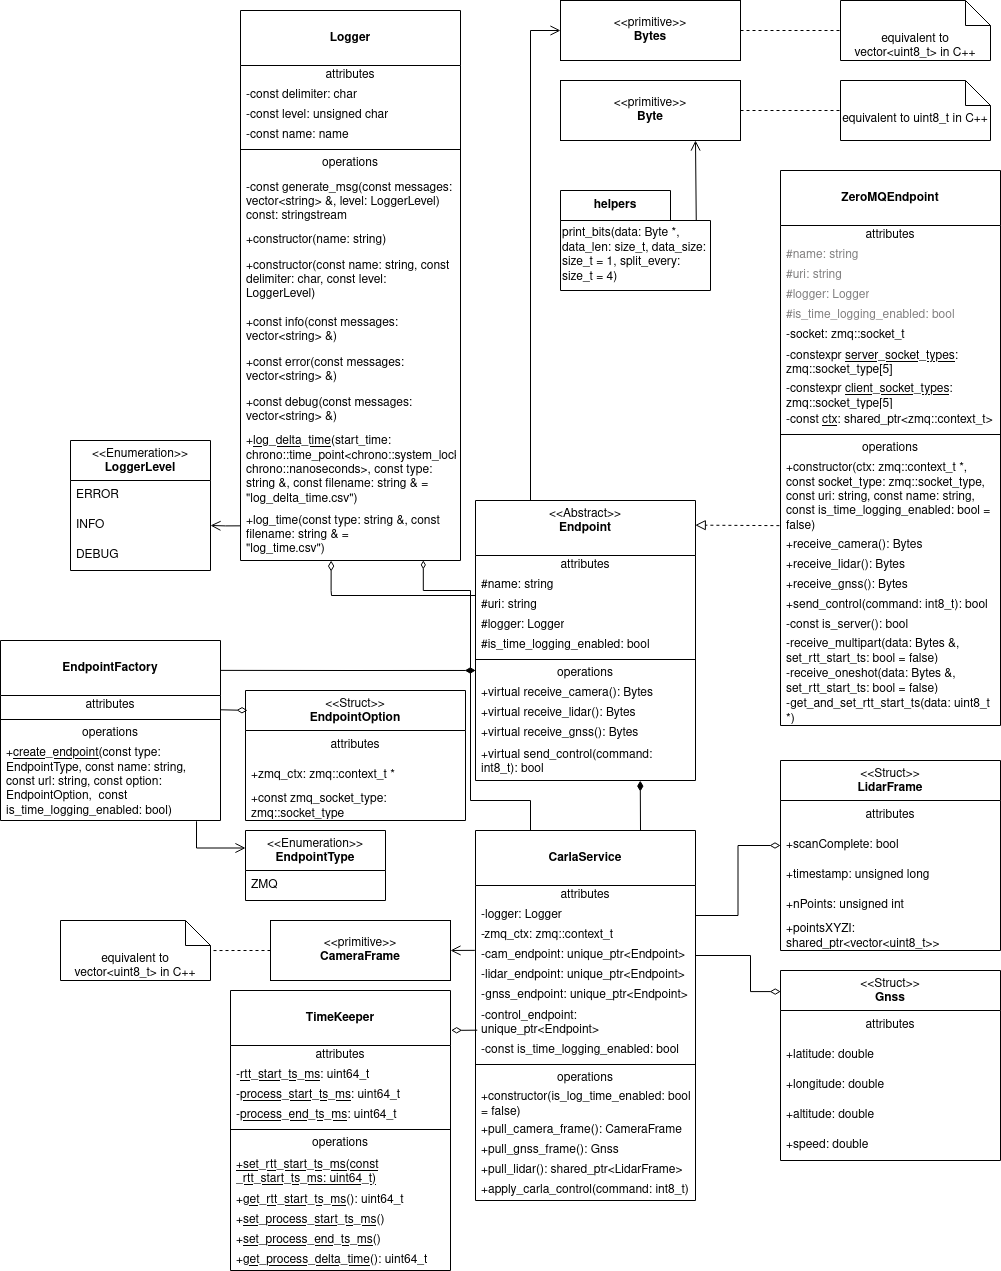
\includegraphics[width=1.0\textwidth]{resources/chapter-4/consumer-class_diagram.png}
	\caption{Diagram Kelas Pustaka \textit{Consumer}}
	\label{chapter-4-consumer-class-diagram}
\end{figure}

Setelah pustaka \textit{consumer} berhasil, implementasi dilanjutkan dengan
pembuatan pustaka \textit{producer}. Diagram kelas pustaka \textit{producer}
dapat dilihat pada gambar \ref{chapter-4-producer-class-diagram}. Pembuatan
pustaka \textit{producer} juga mengikuti filosofi penulisan pustaka
\textit{consumer}. Pustaka dibuat seabstrak mungkin sehingga tidak
\textit{coupled} dengan trem. Kelas \texttt{Endpoint} juga dibuat abstrak agar
dapat ditambahkan metode komunikasi yang lain. Perbedaan implementasi adalah
pada kelas yang berinteraksi dengan program utama. Pada pustaka
\textit{producer}, ada empat kelas yang berinteraksi dengan program utama, yaitu
\texttt{CameraHandler}, \texttt{LidarHandler}, \texttt{GnssHandler}, dan
\texttt{ControlHandler}. Keempat kelas memiliki peran masing-masing dan
terspesialisasi untuk menangani data dari sensor virtual CARLA tertentu.
\begin{figure}[!htbp]
	\centering
	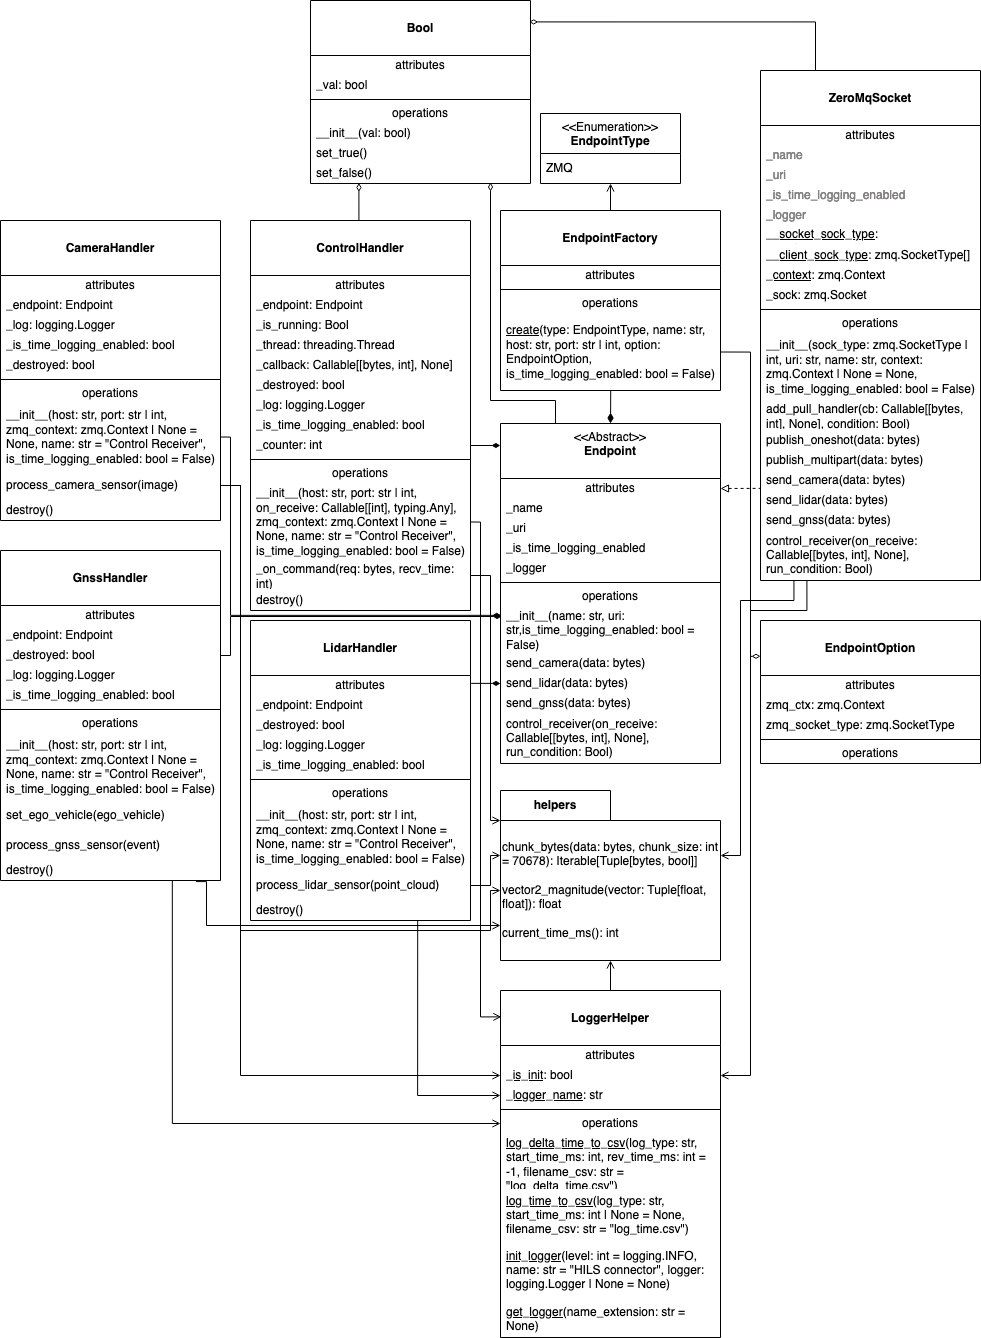
\includegraphics[width=1.0\textwidth]{resources/chapter-4/producer-class_diagram.png}
	\caption{Diagram Kelas Pustaka \textit{Producer}}
	\label{chapter-4-producer-class-diagram}
\end{figure}

Setelah kedua pustaka diimplementasi, dilakukan pengujian pustaka dengan program
kecil. Lalu, kedua pustaka diintegrasi dengan kedua program utama. Setelah itu,
dapat dianggap sistem implementasi HILS yang baru sudah diimplementasi dan
pengujian HILS dapat dilakukan. Akan tetapi untuk kebutuhan tugas akhir, sebelum
pengujian HILS dilakukan, akan dilaksanakan pengujian. Metode pengujian dan
aspek sistem yang diuji akan dibahas pada Subbab
\ref{chapter-4-testing-methodology}.

\section{Metode Pengujian Implementasi dan
  Kinerja}\label{chapter-4-testing-methodology}

Pengujian akan menguji dua aspek, yaitu
\begin{enumerate}
	\item pengujian implementasi: meninjau kemampuan sistem HILS dalam mengirim,
	      menerima, dan menggunakan data dari sensor; dan
	\item pengujian kinerja: meninjau latensi yang dibutuhkan untuk mengirim
	      data.
\end{enumerate}
Bagian ini, Subbab \ref{chapter-4-testing-methodology}, akan membahas metode dan
rencana pengujian kedua aspek tersebut. Pengujian dilakukan dengan menjalankan
beberapa skenario simulasi lalu dibandingkan dengan kriteria kedua aspek. Sebuah
aspek dinyatakan berhasil/lolos apabila semua kriterianya berhasil dicapai.

\subsection{Pengujian Implementasi Sistem HILS}

Pengujian implementasi dilakukan dengan menjalankan program utama di komputer
SILS dan komputer AGX/RKB. Kemudian, akan dilakukan observasi untuk memeriksa
sistem HILS sudah memenuhi kriteria-kriteria pada tabel
\ref{chapter-4-tbl-impl-criteria} atau belum.
\begin{table}[!htbp]
	\begin{center}
		\begin{tabular}{|l|l|}
			\hline
			\textbf{Kode} & \textbf{Deskripsi}                                     \\
			\hline
			IMPL-01       & Kecepatan trem di program GRS sesuai dengan bacaan
			sensor                                                                 \\
			              & GNSS.                                                  \\
			\hline
			IMPL-02       & Tampilan kamera di program GRS sesuai dengan yang
			ada di                                                                 \\
			              & program ScenarioRunner.                                \\
			\hline
			IMPL-03       & Tampilan lidar di program GRS menampikan
			objek-objek                                                            \\
			              & yang ada di sekitar trem.                              \\
			\hline
			IMPL-04       & Trem maju ketika mendapatkan kendali maju dan berhenti \\
			              & ketika mendapatkan kendali berhenti.                   \\
			\hline
		\end{tabular}
	\end{center}

	\caption{Kriteria pengujian implementasi sistem HILS}
	\label{chapter-4-tbl-impl-criteria}
\end{table}

Kriteria ini selaras dengan tujuan tugas akhir yang kedua, yaitu
mengimplementasikan sistem simulasi yang dapat mengirimkan, menerima, dan
memanfaatkan data dari berbagai jenis sensor.

\subsection{Pengujian Kinerja Sistem HILS}

Dari segi kinerja, hal yang ingin dipastikan adalah CARLA dapat berjalan stabil
dengan kecepatan minimum 2 FPS (\textit{frames per second}). Hal tersebut
diobservasi dengan menjalankan kedua program utama. Selain dari kecepatan
simulator, aspek kinerja juga akan dinilai dari perbandingan dengan sistem HILS
yang ada. Latensi pengiriman data harus lebih rendah dibandingkan latensi sistem
HILS yang ada. Kedua kriteria tersebut dituangkan pada tabel
\ref{chapter-4-tbl-perf-criteria}.
\begin{table}[!htbp]
	\begin{center}
		\begin{tabular}{|l|l|}
			\hline
			\textbf{Kode} & \textbf{Deskripsi}                                       \\
			\hline
			PERF-01       & CARLA dapat berjalan dengan stabil dengan kecepatan      \\
			              & minimum 2 FPS.                                           \\
			\hline
			PERF-02       & Latensi pengiriman data lebih rendah dibandingkan sistem \\
			              & HILS yang ada.                                           \\
			\hline
		\end{tabular}
	\end{center}
	\caption{Kriteria pengujian kinerja sistem HILS}
	\label{chapter-4-tbl-perf-criteria}
\end{table}

Pengujian kriteria PERF-02 akan menggunakan \textit{round-trip time} (RTT) yang
dibagi dua untuk perkiraan latensi sistem. Rumus perhitungan RTT dapat dilihat
pada persamaan \ref{chapter-4-eq-rtt}.
\begin{equation}
	\label{chapter-4-eq-rtt}
	\text{RTT} = T_{e} - T_{s} - t_p
\end{equation}

Dengan keterangan persamaan sebagai berikut.
\begin{table}[!h]
	\begin{tabular}{l l}
		RTT     & :     \textit{round-trip time} (dalam ms)             \\
		$T_{e}$ & : \textit{timestamp} didapatkan kendali (dalam ms)    \\
		$T_{s}$ & : \textit{timestamp} dikirimkan segmen pertama kamera
		(dalam ms)                                                      \\
		$t_p$   & :   waktu pemrosesan (dalam ms)
	\end{tabular}
\end{table}

Untuk perhitungan RTT digunakan sensor kamera karena sensor kamera memiliki
ukuran terbesar sehingga diharapkan dapat menjadi kasus terburuk untuk mekanisme
komunikasi. Selain itu, dilakukan dari segmen pertama agar latensi yang dihitung
adalah latensi keseluruhan pengiriman data kamera, tidak hanya sebuah segmen.

Selain itu, pengujian kriteria PERF-02 untuk implementasi HILS sebelumnya akan
dilakukan secara teoretis. Hal ini karena implementasi HILS sebelumnya sudah
sulit untuk dijalankan. Selain itu, jenis data yang dikirim pada implementasi
HILS sebelumnya juga berbeda. Pengujian secara teoretis ini dilakukan dengan
menulis ulang sebagian dari mekanisme komunikasi implementasi HILS sebelumnya.
Bagian yang akan ditulis ulang adalah operasi pembacaan data dari \textit{file},
penulisan dan pembacaan ke basis data, serta penulisan data sensor yang dibaca
dari basis data ke \textit{file}. Dengan demikian, ada 4 operasi I/O dari
implementasi HILS sebelumnya yang ditulis ulang untuk pengujian latensi secara
teoretis.

Apabila sistem HILS berhasil memenuhi kedua kriteria tersebut, sistem dapat
dianggap sudah berhasil memenuhi kedua tujuan tugas akhir. Hal tersebut karena
kinerja sistem akan dipengaruhi mekanisme komunikasi yang digunakan (tujuan
pertama) dan juga cara pustaka di sistem HILS menserialisasi (mengirim) dan
mendeserialisasi (menerima) data sensor (tujuan kedua).

\section{Hasil Pengujian}

Penjabaran hasil pengujian aspek implementasi dan kinerja akan dipisah.
Penjabaran dipisah karena hal yang diujikan serta kriteria pengujian dari kedua
aspek berbeda.

\subsection{Hasil Pengujian Implementasi Sistem HILS}

Dari pengujian yang dilakukan, ditemukan bahwa sistem HILS dapat memenuhi
seluruh kriteria yang untuk pengujian implementasi sistem. Penjabaran
ketercapaian kriteria pengujian implementasi sistem HILS dapat dilihat pada
\ref{chapter-4-tbl-impl-criteria-result}. Selain itu, tampilan sistem HILS dan
hasil implementasi dapat dilihat pada gambar \ref{chapter-4-fig-hils-running}.

Pada gambar \ref{chapter-4-fig-hils-running}, dapat dilihat sistem simulasi
sudah dijalankan di komputer AGX dan komputer SILS. Komputer SILS ditampilkan di
komputer sebelah kiri menggunakan bantuan program AnyDesk. Seperti yang
terlihat, sistem simulasi sudah berjalan dengan baik. Tampilan kamera di program
ScenarioRunner (SILS) dan program GRS (AGX) sudah sama.

\begin{table}[!htbp]
	\begin{center}
		\begin{tabular}{|l|l|l|}
			\hline
			\textbf{Kode} & \textbf{Deskripsi}                         & \textbf{Tercapai} \\
			\hline
			              & Kecepatan yang ditampilkan GUI pada        &                   \\
			IMPL-01       & program ScenarioRunner dan pada program    & \checkmark        \\
			              & GRS sudah sama.                            &                   \\
			\hline
			IMPL-02       & Frame kamera yang tampil pada GUI program  & \checkmark        \\
			              & ScenarioRunner dan program GRS sudah sama. &                   \\
			\hline
			IMPL-03       & Data dari lidar sudah menampilkan objek    & \checkmark        \\
			              & sekitar trem di GUI program GRS.           &                   \\
			\hline
			              & Trem di CARLA sudah dapat bergerak tanpa   &                   \\
			IMPL-04       & butuh masukan di program ScenarioRunner    & \checkmark        \\
			              & dan sesuai dengan luaran kendali dari      &                   \\
			              & program GRS.                               &                   \\
			\hline
		\end{tabular}
	\end{center}

	\caption{Tercapainya pengujian implementasi atau tidak.}
	\label{chapter-4-tbl-impl-criteria-result}
\end{table}

\begin{figure}[!htbp]
	\centering
	\includegraphics[width=1.0\textwidth,trim={12cm 12cm 0 12cm},clip]{resources/chapter-4/HILS-system-running.png}
	\caption{Tampilan sistem HILS ketika dijalankan. Tampilan komputer SILS di
		sebelah kiri, tampilan komputer AGX di sebelah kanan.}
	\label{chapter-4-fig-hils-running}
\end{figure}

\subsection{Hasil Pengujian Kinerja Sistem HILS}

Hasil pengujian kinerja sistem HILS dapat dilihat pada tabel \ref{chapter-4-tbl-perf-criteria-result}.

\begin{table}[!htbp]
	\begin{center}
		\begin{tabular}{|l|l|l|}
			\hline
			\textbf{Kode} & \textbf{Deskripsi}                                  & \textbf{Tercapai} \\
			\hline
			              & Sistem HILS gagal memiliki kinerja yang baik ketika &                   \\
			PERF-01       & sensor lidar digunakan, CARLA gagal mencapai        & X$^*$             \\
			              & 2 FPS. Akan tetapi, tanpa sensor lidar bisa         &                   \\
			              & mencapai lebih dari 10 FPS.                         &                   \\
			\hline
			              & Sistem HILS baru berhasil memiliki kinerja yang     &                   \\
			PERF-02       & lebih baik daripada sistem HILS sebelumnya. Namun,  & \checkmark$^*$    \\
			              & pelaksanaan pengujian PERF-02 dilakukan tanpa       &                   \\
			              & sensor lidar, hanya sensor kamera dan GNSS.         &                   \\
			\hline
		\end{tabular}
	\end{center}

	\caption{Tercapainya pengujian implementasi atau tidak.}
	\label{chapter-4-tbl-perf-criteria-result}
\end{table}

Kriteria PERF-01 gagal dipenuhi seluruhnya dikarenakan ketika menggunakan sensor
lidar kinerja sistem buruk. Akan tetapi, ketika sensor lidar ``dihilangkan,''
kinerja menjadi sangat baik bahkan CARLA dapat melebihi 10 FPS. Sedangkan
kriteria PERF-02 bisa dianggap berhasil dipenuhi dengan catatan pengujian
PERF-02 tanpa sensor lidar.

Data pengujian kinerja dapat dilihat pada Lampiran
\ref{appendix-performance-data}. Selain itu, program Jupyter Notebook yang
digunakan untuk pemrosesan data kinerja dapat dilihat pada lampiran
\ref{appendix-algoritma-monitoring}.

\section{Pembahasan}
\blindtext
